\documentclass{article}

\usepackage[english]{babel}
\usepackage[utf8]{inputenc}
\usepackage{polski}
\usepackage[T1]{fontenc}
 
\usepackage[margin=1.5in]{geometry} 

\usepackage{color} 
\usepackage{amsmath}
\usepackage{amsfonts}                                                                   
\usepackage{graphicx}                                                             
\usepackage{booktabs}
\usepackage{amsthm}
\usepackage{pdfpages}
\usepackage{wrapfig}
\usepackage{hyperref}
\usepackage{etoolbox}
\usepackage{tikz}

\makeatletter
\newenvironment{definition}[1]{%
    \trivlist
    \item[\hskip\labelsep\textbf{Definition. #1.}]
    \ignorespaces
}{%
    \endtrivlist
}
\newenvironment{fact}[1]{%
    \trivlist
    \item[\hskip\labelsep\textbf{Fact. #1.}]
    \ignorespaces
}{%
    \endtrivlist
}
\newenvironment{theorem}[1]{%
    \trivlist
    \item[\hskip\labelsep\textbf{Theorem. #1.}]
    \ignorespaces
}{%
    \endtrivlist
}
\newenvironment{information}[1]{%
    \trivlist
    \item[\hskip\labelsep\textbf{Information. #1.}]
    \ignorespaces
}{%
    \endtrivlist
}
\newenvironment{identities}[1]{%
    \trivlist
    \item[\hskip\labelsep\textbf{Identities. #1.}]
    \ignorespaces
}{%
    \endtrivlist
}
\makeatother

\title{Programowanie Funkcyjne}  
\author{Rafał Włodarczyk}
\date{INA 4, 2025}

\begin{document}

\maketitle

\tableofcontents

\section{Lecture I - Haskell}

Haskell = leniwy język funkcyjny\\

\[
    \textit{functions are first class objects}
\]

\[
    x \rightarrow \fbox{f} \rightarrow f(x)
\]

\noindent
Rozważmy fragment kodu:
\begin{verbatim}
int c = 2;
int f(int x) {
    return (c*x);
}
\end{verbatim}
Ta funkcja nie jest czysta - wykorzystuje swoje środowisko.\\\\
Rozważmy fragment kodu:
\begin{verbatim}
int f(int x) {
    printf("Hello");
    return (2 * x);
}
\end{verbatim}
Zadziała na środowisku zewnętrznym - to nie jest czysta funkcja
\begin{verbatim}
int f(int x) {
    return (2*x);
}
\end{verbatim}
Nie wpływa na otoczenie, nie wykorzystuje, ani nie zmienia występujacych obiektów.\\
Języki funkcyjne operują na czystych funkcjach.

\subsection{Instalacja Haskella - GHCup}

\textit{ghci} - interaktywna konsola GHC (Glasgow Haskell Compilers)

\begin{verbatim}
ghci> 1 + 2
3
ghci> :? # help
ghci> :q # exit
ghci> :load file.hs
\end{verbatim}

\subsection{Problem wczytywania zmiennych}

\begin{verbatim}
!! readInt() {...} :: Int
\end{verbatim}

\begin{definition}{Funkcja jednej zmiennej}.\\

\noindent
Zdefiniujmy funkcję

\begin{verbatim}
w1.hs

f x = 1 + x*(1+x)

ghci>:load w1
ghci>f 1
3
ghci>:type f
f :: Num a => a -> a
ghci>:info Num 
\end{verbatim}
Podstawowy typ Num
\begin{verbatim}
ghci> :info Num
type Num :: * -> Constraint
class Num a where
    (+) :: a -> a -> a
    (-) :: a -> a -> a
    (*) :: a -> a -> a
    negate :: a -> a
    abs :: a -> a
    signum :: a -> a
    fromInteger :: Integer -> a
    {-# MINIMAL (+), (*), abs, signum, fromInteger, (negate | (-)) #-}
        -- Defined in ‘GHC.Num’
instance Num Double -- Defined in ‘GHC.Float’
instance Num Float -- Defined in ‘GHC.Float’
instance Num Int -- Defined in ‘GHC.Num’
instance Num Integer -- Defined in ‘GHC.Num’
instance Num Word -- Defined in ‘GHC.Num’
\end{verbatim}
\end{definition}

\subsection{Podstawowe typy}

Int, Integer (unlimited size), Float, Double, Char, Bool

\[
\text{Int, Integer} \in \text{Integral} \subseteq \text{Num}
\]

\begin{center}
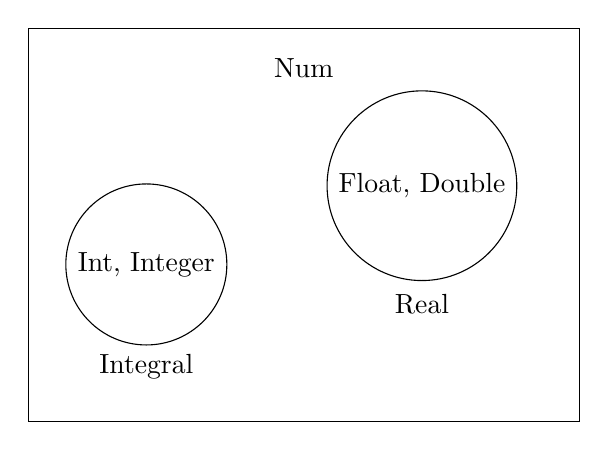
\begin{tikzpicture}
    \node at (3.5,4.5) {Num};
    \draw (0,0) rectangle (7, 5);
    \node at (1.5,2) [circle, draw] {Int, Integer};
    \node at (1.5, 0.7) {Integral};
    \node at (5, 3) [circle, draw] {Float, Double};
    \node at (5, 1.5) {Real};
\end{tikzpicture}
\end{center}

\noindent
Pod spodem działa \href{https://en.wikipedia.org/wiki/Hindley%E2%80%93Milner_type_system}{Teoria Typowania Hindleya - Milnera}

\begin{verbatim}
f(3.23 :: Double) # możemy explicite wymusić typ
\end{verbatim}

\begin{center}
    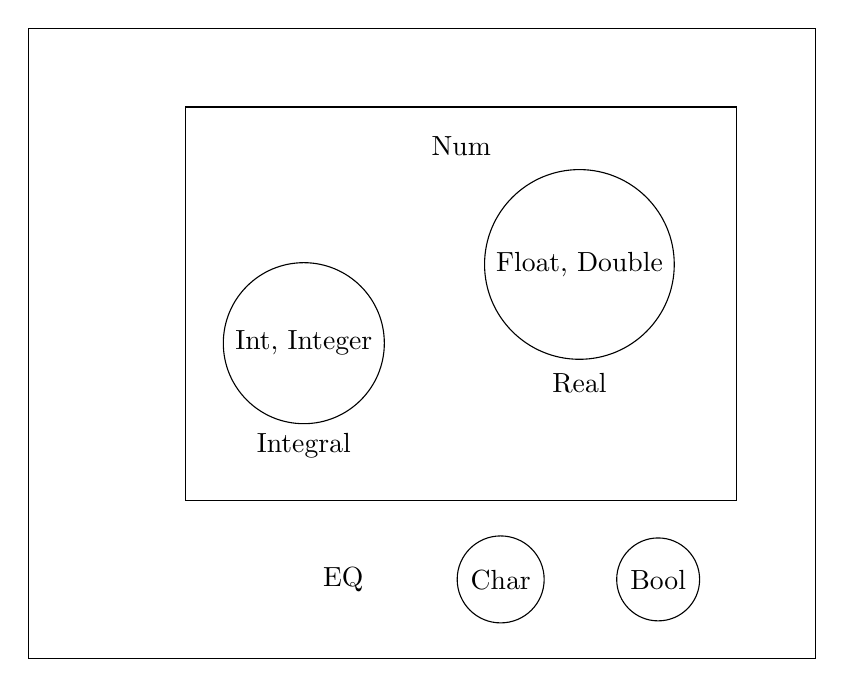
\begin{tikzpicture}
        \draw (-2,-2) rectangle(8, 6);
        \node at (2, -1)  {EQ};
        \node at (4, -1)  [circle, draw] {Char};
        \node at (6, -1)  [circle, draw] {Bool};
        \node at (3.5,4.5) {Num};
        \draw (0,0) rectangle (7, 5);
        \node at (1.5,2) [circle, draw] {Int, Integer};
        \node at (1.5, 0.7) {Integral};
        \node at (5, 3) [circle, draw] {Float, Double};
        \node at (5, 1.5) {Real};
    \end{tikzpicture}
\end{center}

\begin{definition}{w1.hs} Zdefiniujmy funkcje:\\

\begin{verbatim}
ghci> g x y = 1 + x * y
ghci> :type g
g :: (Fractional t1, Num a) => t1 -> t2 -> a
ghci> g x y = 1 + x * y
ghci> h = g (2::Int)
ghci> :t h
h :: Int -> Int
\end{verbatim}
\end{definition}
Z podobną sytuacją mieliśmy do czynienia przy potęgowaniu liczb kardynalnych:
\begin{align}
    \left| C^{B\times A} \right| = \left| \left(C^B\right)^A \right| 
\end{align}
    
\subsection{$\lambda$-wyrażenie}

\begin{definition}{$\lambda$-wyrażenie (funkcja anonimowa)}
\[
    \left(\lambda x \rightarrow \text{expr}\right)(t) = \text{expr}\left[x\leadsto  t\right]
\]
Chcielibyśmy znaleźć:
\begin{align}
\Psi &: C^{B\times A} \rightarrow \left(C^B\right)^A\\
\Psi (t) &= \left(\lambda a : A \rightarrow \left(\lambda b: B \rightarrow f (a,b) \right)\right)\\
\Psi (f) (a) &= (\lambda b : B \rightarrow f(a,b))
\end{align}
Funkcję $\Psi$ nazywamy funkcją curry. Wszyskie funkcje w Haskellu są poddane curryingowi.\\

\textit{Curry Haskell - Amerykański Logik z XX wieku.}\\

\end{definition}

\noindent
Podstawowym narzędziem języków funkcyjnych jest rekursja.

\begin{information}{Silnia}
Zapiszmy silnię w Haskellu. Najsilniejsze działanie w Haskellu to aplikacja funkcji na argumencie:
\begin{verbatim}
fact1 n = if n == 0 then 1 
          else n * fact1 (n - 1);
\end{verbatim}
\textit{else} musi być w Haskellu - wynik zawsze musi być czymś.
\end{information}


\begin{information}{Pattern Matchings}
Zapiszmy lepszą silnie:
\begin{verbatim}
fact2::Integer -> Integer
fact2 0 = 1
fact2 n = n * fact2(n-1)
\end{verbatim}
\end{information}

\begin{information}{Case Expression}
Zapiszmy za pomocą case expression:
\begin{verbatim}
fact3 n = case n of
          0 -> 1
          otheriwse -> n * fact3(n-1) 
\end{verbatim}
\end{information}

\begin{information}{Pseudozmienne}
Zapiszmy pseudozmienne:
\begin{verbatim}
fact4 n = let y = n - 1 in
        if n == 0 then 1
        else n * fact4 y

fact4 n = (lambda y -> if n==0 then 1 else n * fact4 y)(n-1)
\end{verbatim}
\end{information}
To jest język C
\begin{verbatim}
h x = x + x sin(x) sin^2 (x)
float h(float x) {
    float y = sin(x);
    return (x + x*y + y*y);
}
\end{verbatim}
Równoważnik Haskellowy:
\begin{verbatim}
h x = (\y -> x + x*y + y*y)(sin x)
h x = let y = sin x in 
      x + x*y + y*y
\end{verbatim}

\section{Lecture II}

Zbadajmy identyczność:
\begin{verbatim}
    id:: a -> a
    id:: forall a => a -> a
\end{verbatim}
Lambda kwantyfikuje typy, a nie zmienne - głębokie znaczenie polimorfizmu\\
\begin{align}
    \exp &= \left(\lambda a: \text{Typ} \rightarrow (a\rightarrow a)\right)\\
    \exp & (\text{Int}) :: \text{Int} \rightarrow \text{Int}\\
    \exp & (\text{Double}) :: \text{Double} \rightarrow \text{Double}
\end{align}

\begin{verbatim}
ghci> inc x = x + 1
ghci> :t inc
inc :: Num a => a -> a
\end{verbatim}

\begin{align}
    \exp = (\forall a: \text{Num} \rightarrow (a\rightarrow a))    
\end{align}
Zasada: \textit{W linijce przed wyrażeniem opisuje jego typ.}

\subsection{Tworzenie własnych typów}

\begin{enumerate}
    \item pary
    \item listy
\end{enumerate}

\subsection{Pary}

\begin{verbatim}
ghci> :t (13, 'a')
(13, 'a') :: Num a => (a, Char)
ghci> :t (13::Integer, 'a')
(13::Integer, 'a') :: (Integer, Char)
\end{verbatim}

\begin{verbatim}
coll n = | n == 1 then 1
         | even n then call (div n 2)  -- n `div` 2
         | otherwise call (3*n + 1)

collatz :: (Int, Int) -> (Int, Int)
collatz (n, s) | n == 1 = (n, s)
            | even n = collatz (div n 2, s + 1)
            | otherwise = collatz (3 * n + 1, s + 1)
\end{verbatim}

\subsection{Listy}

\begin{verbatim}
[a] =    elementów a
\end{verbatim}

\begin{align}
    \{[a_1,\dots,a_k]: a_1,\dots,a_k, a_i\in a, k\in \mathbb{N}\}
\end{align}

\begin{verbatim}
[1,2,3]

[1,_]->[2, ]->[3, ]->[ ]
x_0: [x_1, x_2, ..., x_k] = [x_0, x_1, ... x_k]
[] <- lista pusta
[1,2,3] ~= 1:2:3:[]
konkatenacja dwóch list ++
[1,2,3] ++ [4,5,6] = [1,2,3,4,5,6]

concat :: [[a]] -> [a]
concat [[1,2,3],[5],[0,1]] = [1,2,3,4,0,1]

length :: [a] -> Int
length [] = 0
length (x:xs) = 1 + length xs -- x, xs (some x-es)

aplikacja funkcji do zmiennej ma najwyższy priorytet
f x = ...

[] ++ ys = ys
(x:xs)++ys = x:(xs++ys)
[1,2]++[] = 1:([2]++[]) = 1:(2:([]||[])) = [1,2]

head [] = error bad: pusta lista
head (x:_) = x

tail [] = []
tail (x:xs) = xs

-- mapowanie
[x_1,x_2,...x_k], f: a -> b
[fx_1,fx_2... fx_k]

map::(a->b)->[a]->[b]
map _ [] = []
-- ciąg którego głowa to jest x, a ogon to xs
map f (x:xs) = f x : map f xs

map(\x -> x^2)[1..10] -> [1^2, 2^2, ..., 100]

-- filtrowanie

filter::(a->Bool)->[a]->[a]
filter even [1..10] -> [2,4,6,8,10]

filter _ [] = []
filter p (x:xs) = if p x then x:filter p xs
                  else filter p xs

-- prototypy

list comprehension

[f x_1 x_2 x_3 | x_1 <- xs, x_2 <- ys, x_3 <- zs]
[f x_1 x_2 x_3 | x_1 <- xs, x_2 <- ys, x_1<x_2, x_3 <- zs]

# wszystkie trójki pitagorejskie do 100
[(x,y,z) | z <- [1..100] y<-[1..z], x<-[1..y], x^2+y^2==z^2, gcd(x,y)==1]

\end{verbatim}

\section{Lecture III}

\texttt{Prelude} - zestaw funkcji automatycznie ładowanych.

Typ wbudowany:
\begin{verbatim}
    type String = [Char]
\end{verbatim}

\subsection{Sortowanie}

\begin{verbatim}
    {- SORTOWANIA -}
    -- quicksort
    qS [] = []
    qS (x:xs) = (qS [y| y <- xs, y < x]) ++
                [x] ++
                (qS [y| y <- xs, y >= x])
    
    -- partition
    partition :: (a -> Bool) -> [a] -> ([a], [a])
    partition _ [] = ([], [])
    partition p (x:xs) = if p x then (x:l, r)
                                else (l, x:r)
                            where (l, r) = partition p xs

    -- qSort 
    qSort []     = []
    qSort [x]    = [x]
    qSort (x:xs) = (qSort l) ++ [x] ++ (qSort r)
                   where (l, r) = partition (<x) xs
    
    -- inSort
    inSort []     = []
    inSort (x:xs) = l ++ [x] ++ r
                    where sxs = inSort xs
                          (l, r) = partition (<x) sxs
\end{verbatim}

\subsection{Operacje}

Operacje binarne: $+, -, *, \wedge, :, <$

\texttt{[1..]} - nieskończona lista
\texttt{zipWith (zipWith (+))} - suma 2 macierzy
\begin{verbatim}
    > zipWith (zipWith (+)) [[1,1],[1,1]] [[2,3],[4,5]]
    [[3,4], [5, 6]]
\end{verbatim}

\begin{verbatim}
    add [] = 0
    add (x:xs) = x + add xs
    
    -- product
    pro [] = 1
    pro (x:xs) = x * pro xs
\end{verbatim}

$[x_1, x_2, x_3, x_4], *, e $ to wtedy
$x_1 * (x_2 * (x_3 * (x_4 * e)))$ lub $(((x_1 * e) * x_2) * x_3) *x_4$

\subsection{Monoidy}

Jeśli $*$ jest łączne, a $e$ to element neutralny, to $(X, *, e)$ nazywamy monoidem.

\begin{verbatim}
    myfoldr op e [] = e
    myfoldr op e (x:xs) = op x (myfoldr op e xs)
    
    myfoldl op e [] = e 
    myfoldl op e (x:xs) = myfoldl op (op e x) xs
\end{verbatim}

foldl (*) e [x1, x2, x3, x4]
\begin{verbatim}
        *
       / \
      *  x4
     / \
    *  x3
   / \
  *  x2
 / \
e   x1
\end{verbatim}
foldr (*) e [x1, x2, x3, x4]
\begin{verbatim}
  *
 / \
x1  *
   / \
  x2  *
     / \
    x3  *
       / \
      x4  e

\end{verbatim}
$x \square y = y * x$ \\
$foldl (\square) e [x1, x2, x3, x4]$
\begin{verbatim}
  \square
 / \
x4  \square
   / \
  x3  \square
     / \
    x2  \square
       / \
      x1  e
\end{verbatim}

\noindent
foldl ($\square$) e xs = foldr (*) e (reverse xs)

\noindent
(flip f) x y = f y x \\
reverse xs = foldl (flip(:)) [] xs

\section{Lecture IV}

\subsection{User defined types}

\begin{itemize}
    \item type - synonim na istniejący typ
    \item data
\end{itemize}

\textit{Tworzę grę. W te grę chciałbym załadować ... FIZYKĘ}

\end{document}